\chapter{Conservación de la cantidad de movimiento.}
\section{Teorema del transporte de Reynolds para la cantidad de movimiento.}
Sea un volumen sometido a un conjunto de fuerzas:
%\begin{figure}[H]
%	\centering
%	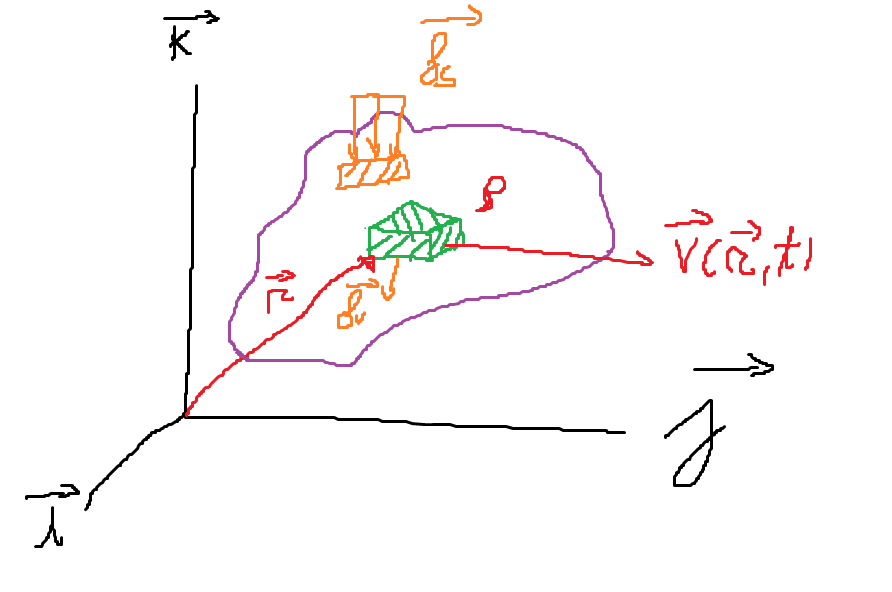
\includegraphics[width=0.7\linewidth]{imagenesTema4/magnitudesFuerzas}
%	\caption{Magnitudes principales que influencian la cantidad de movimiento.}
%	\label{fig:magnitudesfuerzas}
%\end{figure}

\begin{figure}[!ht]
	\centering
		\begin{circuitikz}[scale = 0.9]
			\tikzstyle{every node}=[font=\large]
			\draw [-latex] (-1.75,15.75) -- (-1.75,21.25)node[pos=1,above]{$\vec{k}$};
			\draw [-latex] (-1.75,15.75) -- (5.75,15.75)node[pos=1,right]{$\vec{i}$};
			\draw [-latex] (-1.75,15.75) -- (-3.25,14.25)node[pos=1,left]{$\vec{j}$};
			\draw [ color={rgb,255:red,128; green,0; blue,255}, dashed] (-0.25,20) .. controls (0.5,21.25) and (1.5,20) .. (3,19.75);
			\draw [ color={rgb,255:red,128; green,0; blue,255}, dashed] (3,19.75) .. controls (4,19.75) and (3.25,18.5) .. (3.25,17.25);
			\draw [ color={rgb,255:red,128; green,0; blue,255}, dashed] (3.25,17.25) .. controls (3.5,15.75) and (2.5,16) .. (1,16.25);
			\draw [ color={rgb,255:red,128; green,0; blue,255}, dashed] (1,16.25) .. controls (0,16.75) and (-0.5,16) .. (-0.75,17.25);
			\draw [ color={rgb,255:red,128; green,0; blue,255}, dashed] (-0.75,17.25) .. controls (-1.25,18.75) and (-0.5,19) .. (-0.25,20);
			\node [font=\large, color={rgb,255:red,128; green,0; blue,255}] at (3.75,19.5) {V};
			\draw [ color={rgb,255:red,0; green,128; blue,0} ] (0.5,18.25) rectangle (1.75,17.5);
			\draw [ color={rgb,255:red,0; green,128; blue,0}, short] (0.5,18.25) -- (0.75,18.5);
			\draw [ color={rgb,255:red,0; green,128; blue,0}, short] (0.75,18.5) -- (2,18.5);
			\draw [ color={rgb,255:red,0; green,128; blue,0}, short] (2,18.5) -- (1.75,18.25);
			\draw [ color={rgb,255:red,0; green,128; blue,0}, short] (2,18.5) -- (2,17.75);
			\draw [ color={rgb,255:red,0; green,128; blue,0}, short] (2,17.75) -- (1.75,17.5);
			\draw [ color={rgb,255:red,255; green,0; blue,0}, -latex] (2,18) -- (6.25,18)node[pos=1,above]{$\vec{v}(\vec{r},t)$};
			\draw [ color={rgb,255:red,255; green,128; blue,0}, -latex] (1.25,17.75) -- (1.25,16.5)node[pos=0.85,right]{$\vec{f}_V$};
			\draw [ color={rgb,255:red,255; green,128; blue,0}, short] (0.25,20.25) .. controls (1.25,20.25) and (1.75,19.75) .. (3,19.5);
			\draw [ color={rgb,255:red,255; green,128; blue,0}, short] (3,19.5) -- (2.75,19.25);
			\draw [ color={rgb,255:red,255; green,128; blue,0}, short] (2.75,19.25) .. controls (1.25,19.5) and (1.25,20) .. (0,20);
			\draw [ color={rgb,255:red,255; green,128; blue,0}, short] (0,20) -- (0.25,20.25);
			\draw [ color={rgb,255:red,255; green,128; blue,0}, -latex] (1.5,21.25) -- (1.5,19.75)node[pos=0,above]{$\vec{f}_S$};
			\draw [ color={rgb,255:red,255; green,128; blue,0}, -latex] (2,21) -- (2,19.5);
			\draw [ color={rgb,255:red,255; green,128; blue,0}, -latex] (2.5,20.75) -- (2.5,19.5);
			\draw [ color={rgb,255:red,255; green,128; blue,0}, -latex] (1,21.25) -- (1,20);
			\draw [ color={rgb,255:red,255; green,128; blue,0}, -latex] (0.5,21.25) -- (0.5,20);
			\draw [ color={rgb,255:red,255; green,0; blue,0}, -latex] (-1.75,15.75) -- (1,17.75)node[pos=0.65,above]{$\vec{r}$};
		\end{circuitikz}
	\caption{Magnitudes principales que influencian la cantidad de movimiento.}
	\label{fig:magnitudesfuerzas}
\end{figure}

Aplicando al teorema del transporte de Reynolds la función $\Phi=\rho\vec{v}$ y una similitud con la segunda ley de Newton se obtiene para volúmenes fluidos:
\[\iiint_{V_f}\vec{f}_V\,dV+\oiint_{S_f}\vec{f}_s\,dS=
\dfrac{d}{dt}\iiint_{V_f}\rho\vec{v}\,dV=
\iiint_{V_f}\dfrac{\partial \rho\vec{v}}{\partial t}\,dV+\oiint_{S_f}\rho\vec{v}\left(\vec{v}\cdot\vec{n}\right)\,dS\]

Para un volumen de control:
\[\iiint_{V_c}\vec{f}_V\,dV+\oiint_{S_c}\vec{f}_s\,dS=
\dfrac{d}{dt}\iiint_{V_f}\rho\vec{v}\,dV=
\iiint_{V_c}\dfrac{\partial \rho\vec{v}}{\partial t}\,dV
+\oiint_{S_c}\rho\vec{v}\left[\left(\vec{v}-\vec{v}_c\right)\cdot\vec{n}\right]\,dS\]

En estas expresiones aparecen dos tipos de fuerzas:
\begin{enumerate}
	\item Fuerzas volumétricas $\vec{f}_v$
	\begin{enumerate}
		\item Típicamente son fuerzas relacionadas con campos:
		\[\vec{f}_v=\rho \vec{g}\]
		\item Pueden ser también fuerzas de inercia en sistemas de referencia móviles.
		\item En un gas suelen ser despreciables estas fuerzas.
	\end{enumerate}
	\item Fuerzas superficiales $\vec{f}_s$
	
	\begin{enumerate}
		\item La expresión general de estas fuerzas es:
		\[\vec{f}_s=
		\red{\underbrace{\black -P\vec{n}}_{\text{Presión hidroestática}}}\black
		+
		\red{\underbrace{\black \overline{\overline{\tau}}_v\cdot\vec{n}}_{\text{Esfuerzos viscosos}}}\black
		\]
		\item Siendo el tensor de esfuerzas viscosos (es una ecuación constitutiva, depende del material):
		\[
		\overline{\overline{\tau}}=
		\renewcommand{\arraystretch}{1}
		\begin{bmatrix}
			\tau_{xx} & \tau_{xy} & \tau_{xz}\\
			\tau_{yx} & \tau_{yy} & \tau_{yz}\\	
			\tau_{zx} & \tau_{zy} & \tau_{zz}\\
		\end{bmatrix}
		=2\mu \overline{\overline{\xi}} + \lambda \left(\vec{\nabla}\cdot \vec{v}\right)\overline{\overline{I}}
		\]
		Donde \begin{itemize}
			\item $\mu$ es la viscosidad.
			\item $\lambda$ es la viscosidad volumétrica.
			\item $\overline{\overline{I}}$ es la matriz identidad.
		\end{itemize}
	\end{enumerate}
\end{enumerate}
\section{Ecuaciones de Navier-Stokes.}
Se parte del teorema del transporte de Reynolds:
\begin{equation}
	\label{NS1}
\iiint_{V_f}\vec{f}_V\,dV
+
\oiint_{S_f}\vec{f}_s\,dS
=
\iiint_{V_f}\dfrac{\partial \rho\vec{v}}{\partial t}\,dV
+
\oiint_{S_f}\rho\vec{v}\left(\vec{v}\cdot\vec{n}\right)\,dS
\end{equation}
Desarrollando mediante el teorema de la divergencia de Gauss:
\begin{equation}
	\label{NS2}
	\oiint_{S_f}\vec{f}_s\,dS
	=
	\oiint_{S_f}-P\vec{n}_s\,dS
	+
	\oiint_{S_f}\overline{\overline{\tau}}\cdot\vec{n}_s\,dS
	=
	\iiint_{V_f}-\vec{\nabla}p\,dV
	+
	\iiint_{V_f}\vec{\nabla}\cdot\overline{\overline{\tau}}\,dV
\end{equation}

\begin{equation}
	\label{NS3}
\oiint_{S_f}\rho\vec{v}\left(\vec{v}\cdot\vec{n}\right)\,dS
=
\iiint_{V_f}\vec{\nabla}\cdot\left(\rho \vec{ v} \otimes \vec{v}\right)\,dV
\end{equation}

Juntando las ecuaciones \eqref{NS1}, \eqref{NS2} y \eqref{NS3}:
\[\iiint_{V_f}\vec{f}_V\,dV
+
\iiint_{V_f}-\vec{\nabla}P\,dV
+
\iiint_{V_f}\vec{\nabla}\cdot\overline{\overline{\tau}}\,dV
=
\iiint_{V_f}\dfrac{\partial \rho\vec{v}}{\partial t}\,dV
+
\iiint_{V_f}\vec{\nabla}\cdot\left(\rho \vec{ v} \otimes \vec{v}\right)\,dV
\]

Para un valor $V_f \approx dV$ arbitrariamente pequeño pero no nulo. Se obtiene la ecuación Navier-Stokes en forma conservativa:
\[
\vec{f}_V
-
\vec{\nabla}P
+
\vec{\nabla}\cdot\overline{\overline{\tau}}
=
\dfrac{\partial \rho\vec{v}}{\partial t}
+
\vec{\nabla}\cdot\left(\rho \vec{ v} \otimes \vec{v}\right)
\]

Desarrollando:
\[\vec{f}_V
-
\vec{\nabla}P
+
\vec{\nabla}\cdot\overline{\overline{\tau}}
=
\red{\underbrace{\black \rho\dfrac{\partial\vec{v}}{\partial t}
+
\rho \left(\vec{v}\cdot\vec{\nabla}\right)\vec{v}}_{\dfrac{\rho D\vec{v}}{Dt}}}\]
\black
\[\vec{\nabla}\cdot\overline{\overline{\tau}}
=
\vec{\nabla}\cdot\left(2\mu\overline{\overline{\xi}}\right)
+
\vec{\nabla}\cdot\left[\lambda\left(\vec{\nabla}\cdot\vec{v}\right)\overline{\overline{I}}\right]
=
\vec{\nabla}\cdot\left(2\mu\dfrac{\vec{\nabla}\vec{v}+\left(\vec{\nabla}\vec{v}\right)^T}{2}\right)
+
\lambda\vec{\nabla}\cdot\left[\left(\vec{\nabla}\cdot\vec{v}\right)\overline{\overline{I}}\right]
\]

\[\vec{\nabla}\cdot\overline{\overline{\tau}}
	\stackrel{\mu,\lambda=cte}{=}
	\mu\vec{\nabla}^2\vec{v}+\left(\mu+\lambda\right)\vec{\nabla}\left(\vec{\nabla}\cdot\vec{v}\right)
	\]
	
En fluidos newtonianos se cumple que $\rho,\mu=cte$ con lo cual:
\[\dfrac{\partial \rho}{\partial t}=0; \vec{\nabla}\rho=0; \vec{\nabla}\cdot\vec{v}=0\]

Por tanto, las ecuaciones de Navier-Stokes junto a la conservación de la masa en forma diferencial:
\[\rho\dfrac{\partial \vec{v}}{\partial t}+\rho\left(\vec{v}\cdot\vec{\nabla}\right)\vec{v}=-\vec{\nabla}P+\mu\vec{\nabla}^2\vec{v}+\rho \vec{g}\]
\[\dfrac{\partial \rho}{\partial t} +\vec{\nabla}\cdot\left(\rho\vec{v}\right)=0\]
\section{Número de Reynolds.}
El número de Reynolds es un número adimensional que se emplea para caracterizar el movimiento de un fluido y se define como:
\[Re=\dfrac{\text{Orden de magnitud de la inercia convectiva}}{\text{Orden de magnitud de fuerzas viscosas}}\]
\[Re=\dfrac{|\rho\left(\vec{v}\cdot\vec{\nabla}\right)\vec{v}|}{|\mu\vec{\nabla}^2\vec{v}|}
\stackrel{|\vec{\nabla}|=\dfrac{1}{L_c}}{=}\dfrac{\rho_c v^2_c/L_c}{\mu_c v_c/L^2_c}=\dfrac{\rho_c v_c L_c}{\mu_c}\]
\begin{itemize}
	\item Si Re es elevado, el flujo es de inercia dominante, flujo turbulento.
	\item Si Re es bajo, el flujo es de viscosidad dominante, flujo laminar.
\end{itemize}
\section{Teorema de Bernoulli.}
Se parte de la ecuación de Navier-Stokes en forma diferencial:
\[\rho\dfrac{\partial \vec{v}}{\partial t}+\rho\left(\vec{v}\cdot\vec{\nabla}\right)\vec{v}=-\vec{\nabla}P+\mu\vec{\nabla}^2\vec{v}+ \vec{f}_v\]

Desarrollando:
\[\rho\dfrac{\partial \vec{v}}{\partial t}
+
\rho\vec{\nabla}\dfrac{|\vec{v}|}{2}^2-\rho\vec{v} \times \left(\vec{\nabla}\times\vec{v}\right)
=-\vec{\nabla}P+\mu\vec{\nabla}^2\vec{v}+\vec{f}_v
\]
\newpage
Se supone un líquido incompresible, estacionario, fuerzas de viscosidad despreciables y que las fuerzas volumétricas tienen la siguiente función potencial:
\[\vec{f}_V=-g\vec{\nabla}U_g\]
\[\rho\vec{\nabla}\dfrac{|\vec{v}|}{2}^2
-
\rho\vec{v} \times \left(\vec{\nabla}\times\vec{v}\right)
=
-\vec{\nabla}\left(P+\rho U_g\right)\]

Multiplicando por $\vec{v}$
\[\vec{v}\cdot\left[\rho\vec{\nabla}\dfrac{|\vec{v}|}{2}^2
-
\rho\vec{v} \times \left(\vec{\nabla}\times\vec{v}\right)
=
-\vec{\nabla}\left(P+\rho U_g\right)\right]\rightarrow\vec{\nabla}\left(P+\dfrac{1}{2}\rho|v|^2+\rho U_g\right)=0\]

De esta expresión se deduce que:
\[P+\dfrac{1}{2}\rho|v|^2+\rho U_g=cte\]

En el caso de que el campo potencial gravitatorio sea paralelo al eje z, se obtiene el teorema de Bernoulli:
\[P+\dfrac{1}{2}\rho|v|^2+\rho gz=cte\]